The implemented methodology follows the BCI literature. \\
Work is divided in two main tasks for each subject: 
\begin{itemize}
\item Creation and calibration of a classifier based on "offline" data
\item Classification of "online" data (serving also as a test)
\end{itemize}\noindent
{\Large \textbf{Data manipulation:}}
The provided data is in the form of raw EEG [samples x channels], and since in this state it is not useful for classifications, we used the procedure described in class to compute the corresponding PSD [windows x frequencies x channels].\\
Before applying the actual PSD procedure, the EEG data is first transformed into the laplacian referencing with a filter [channels x channels] (Figure \ref{fig:laplacian_filter}) in order to enhance the localization of the events related to the executed tasks (Figure \ref{fig:code_raw_eeg_lap}).\\

\begin{figure}[h!]
	\begin{center}
		 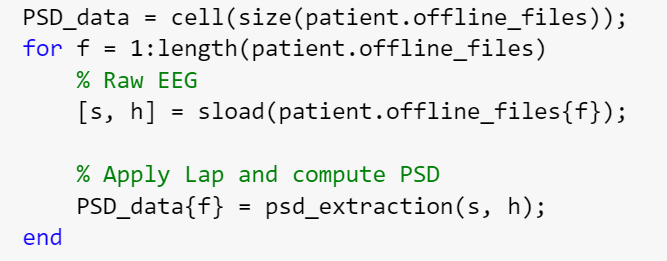
\includegraphics[width=0.4\linewidth]{img/code_raw_eeg_lap.PNG}
	\end{center}

	 \caption{load EEG for offline data - compute Laplacian referencing and PSD for one patient}
	 \label{fig:code_raw_eeg_lap}
\end{figure}

\begin{figure}[h!]
	\begin{center}
		 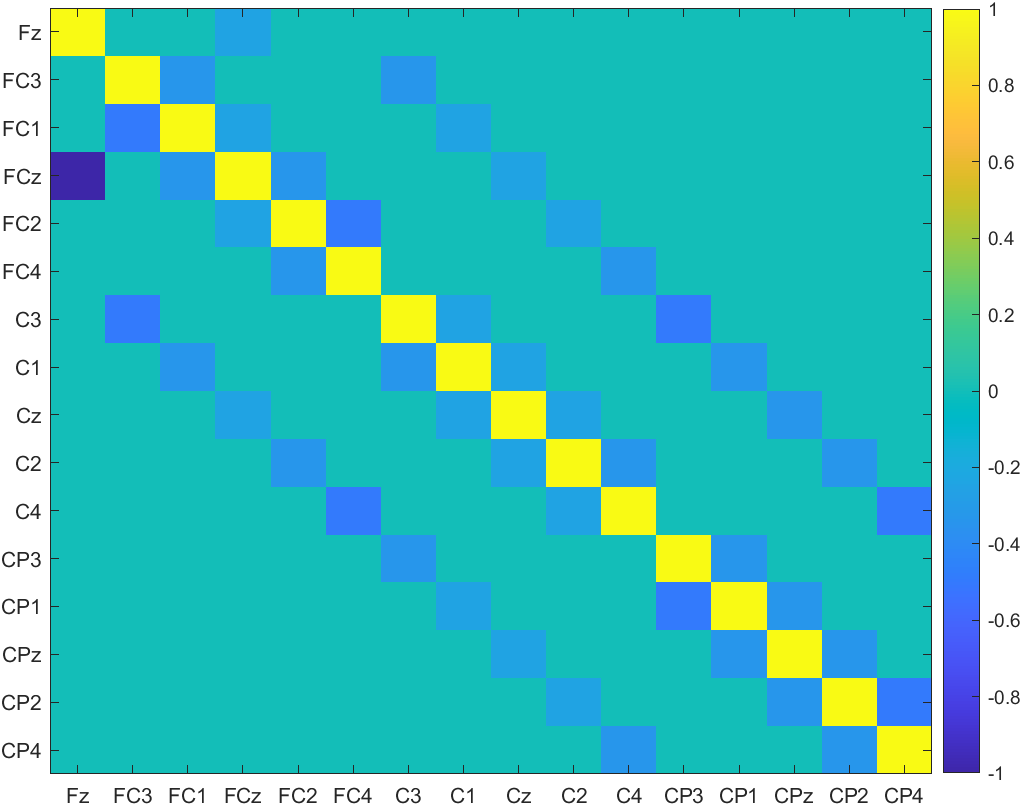
\includegraphics[width=0.5\linewidth]{img/laplacian_filter.png}
	\end{center}

	 \caption{Laplacian filter (16x16)}
	 \label{fig:laplacian_filter}
\end{figure}

After this we have split the data into the offline part used to train an tuning and the online part used as test.\\ \\
{\Large \textbf{Offline task:}}
\begin{itemize}
\item \textbf{Feature selection:}  For each patient, from the data in form of PSD, then the more discriminant features are selected, each feature corresponds to a (frequency , channel) pair. In this step, we take into account only if the pairs that are meaningful for MI tasks that are the beta
\footnote{for beta rhythm we mean the activity of populations of neurons in the motor-cortex region(also frontal region but is not related to motor-imagery tasks) approximately with frequencies 13-30 (can slightly change from subject to subject)}
 and mu
 \footnote{for mu rhythm we mean the activity of populations of neurons in the motor-cortex region approximately with frequencies 8-13 (can slightly change from subject to subject)}
rhythms.\\
In other words:
\begin{itemize}
\item around the channels C3 and C4 for the task of both hands and around Cz for the task of both feet
\item  in the mu band for the ERD
 \footnote{for ERD -event related de synchronization- we mean when some populations of neurons starts to fire in asynchronous way in response to a task to execute causing a decrease in power of the EEG signal in that area}
 in the beta band for the ERS 
 \footnote{for ERS -event related synchronization- we mean when some populations of neurons after an ERD starts to re-synchronize their firing rate causing an increment in power of the EEG signal in that area}
\end{itemize}
In order to correctly select the more discriminant features we have first normalized the distribution of the samples with respect to the two features we are interested in, applying a logarithmic transformation to the PSD matrix (Figure \ref{fig:freq_data_norm}).
Then we computed the Fisher's score (Figure \ref{fig:fisher_score_calibration_ai6}, Figure \ref{fig:fisher_score_avg_filtered_ai6}) and for removing features that from the literature we know are not related to the tasks, we have applied weights (Figure \ref{fig:features_filter}) to them and then selected the best k (Figure \ref{fig:features_selection}).

\textbf{TODO: Justify number of features.}

\begin{figure}[h!]
	\begin{center}
		 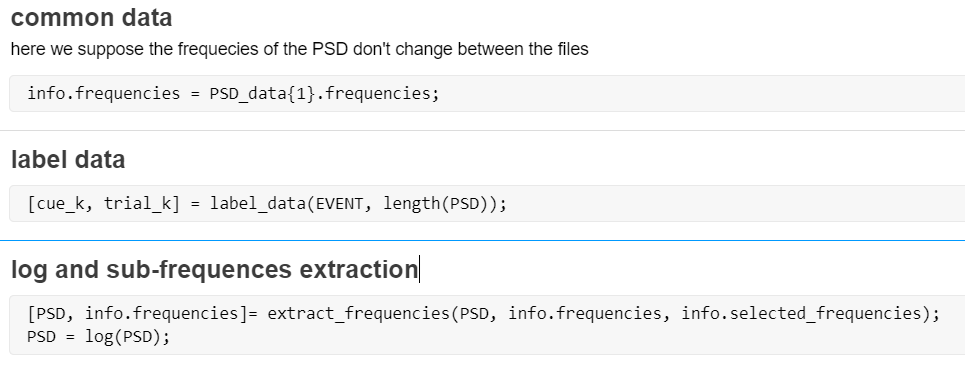
\includegraphics[width=0.6\linewidth]{img/code_extract_frequencies_normalize_data.PNG}
	\end{center}

	 \caption{Extracting frequencies, labeling data and normalization}
	 \label{fig:freq_data_norm}
\end{figure}


\begin{figure}[h!]
	\begin{center}
		 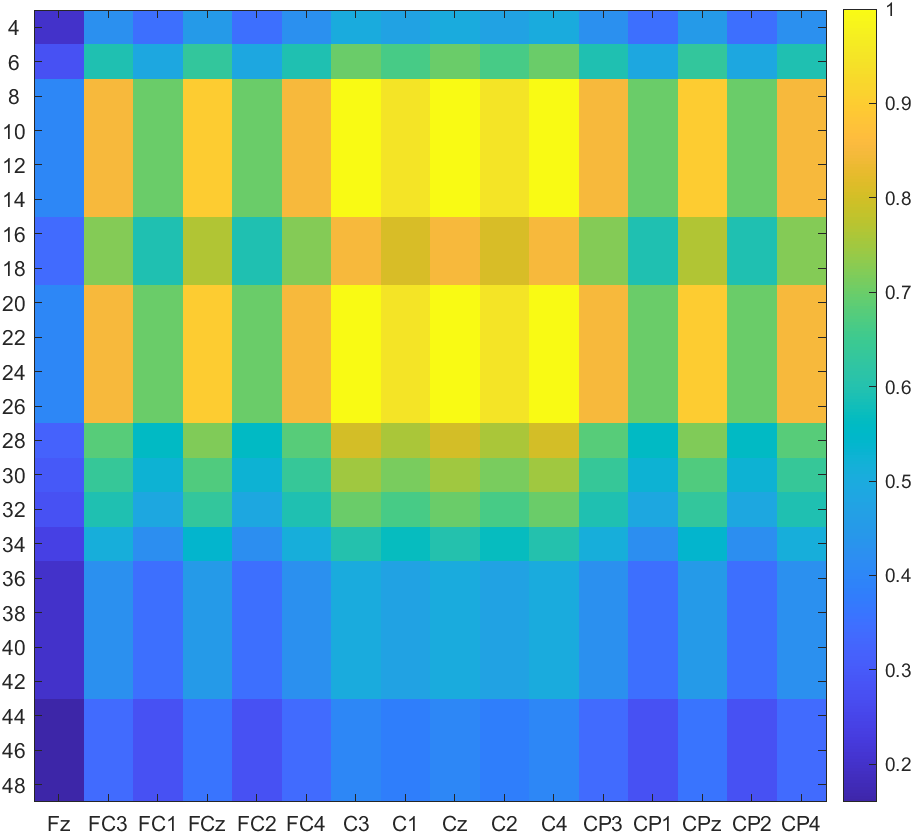
\includegraphics[width=0.4\linewidth]{img/features_filter.png}
	\end{center}

	 \caption{Features filter (23x16) (all patients)}
	 \label{fig:features_filter}
\end{figure}

\begin{figure}[h!]
	\begin{center}
		 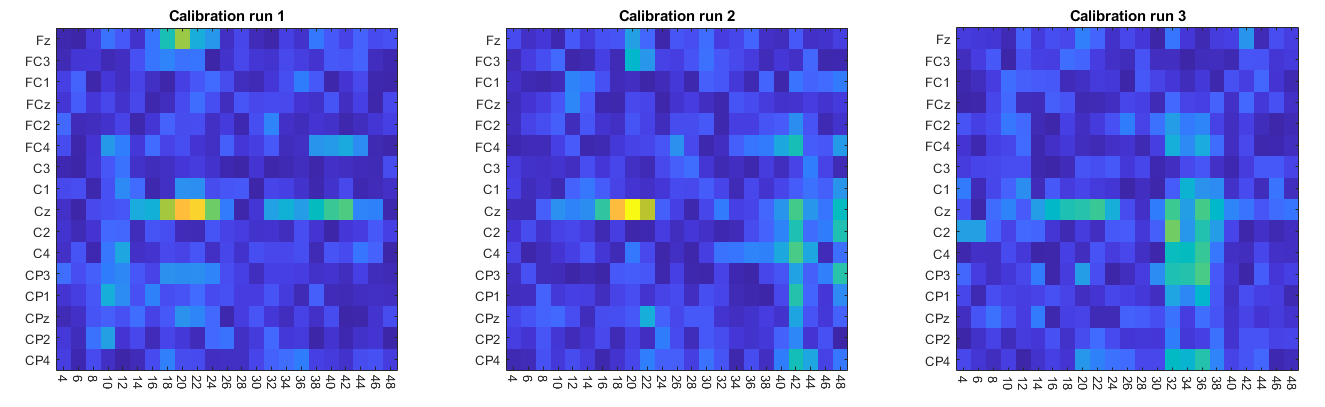
\includegraphics[width=0.8\linewidth]{img/fisher_score_calibration_ai6.PNG}
	\end{center}

	 \caption{Fisher Score (16x23) (subject ai6)}
	 \label{fig:fisher_score_calibration_ai6}
\end{figure}

\begin{figure}[h!]
	\begin{center}
		 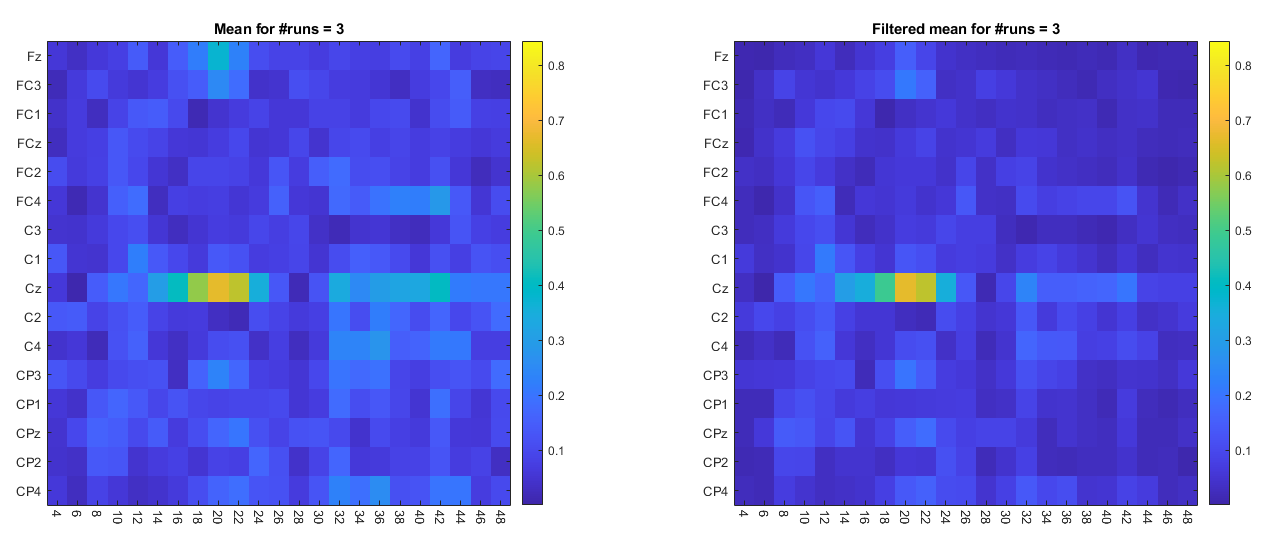
\includegraphics[width=0.8\linewidth]{img/fisher_score_calibration_ai6_avg_filtered.PNG}
	\end{center}

	 \caption{Fisher Score Average on 3 runs and filtered with Features weights (Figure \ref{fig:features_filter}) (16x23) (subject ai6)}
	 \label{fig:fisher_score_avg_filtered_ai6}
\end{figure}



\item \textbf{Classifier training:} The previous steps allow to build a training set for each subject (one can use all the available offline data), by selecting the windows associated with the MI tasks. Then for each subject we applied k-fold cross validation to choose between three differ kind of classificators (LDA, QDA, SVM with rbf kernel).\\

\begin{figure}[h!]
	\begin{center}
		 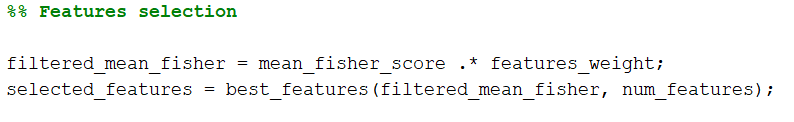
\includegraphics[width=0.8\linewidth]{img/code_select_features.PNG}
	\end{center}

	 \caption{Features selection}
	 \label{fig:features_selection}


	\begin{center}
		 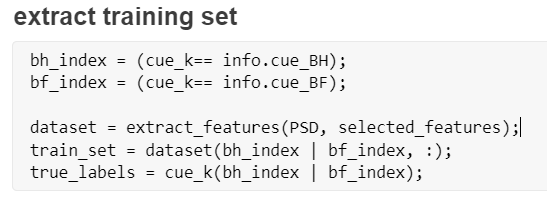
\includegraphics[width=0.5\linewidth]{img/code_extract_train_set.PNG}
	\end{center}

	 \caption{Training set extraction}
	 \label{fig:train_set_extraction}
\end{figure}

\begin{figure}[h!]
	\begin{center}
		 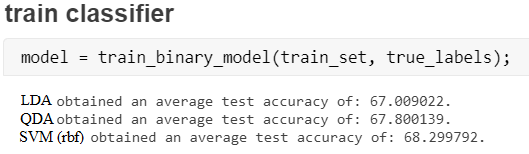
\includegraphics[width=0.5\linewidth]{img/code_cv_ai6.PNG}
	\end{center}

	 \caption{Results of Cross validation on subject ai6}
	 \label{fig:cv_ai6}
\end{figure}

\begin{figure}[h!]
	\begin{center}
		 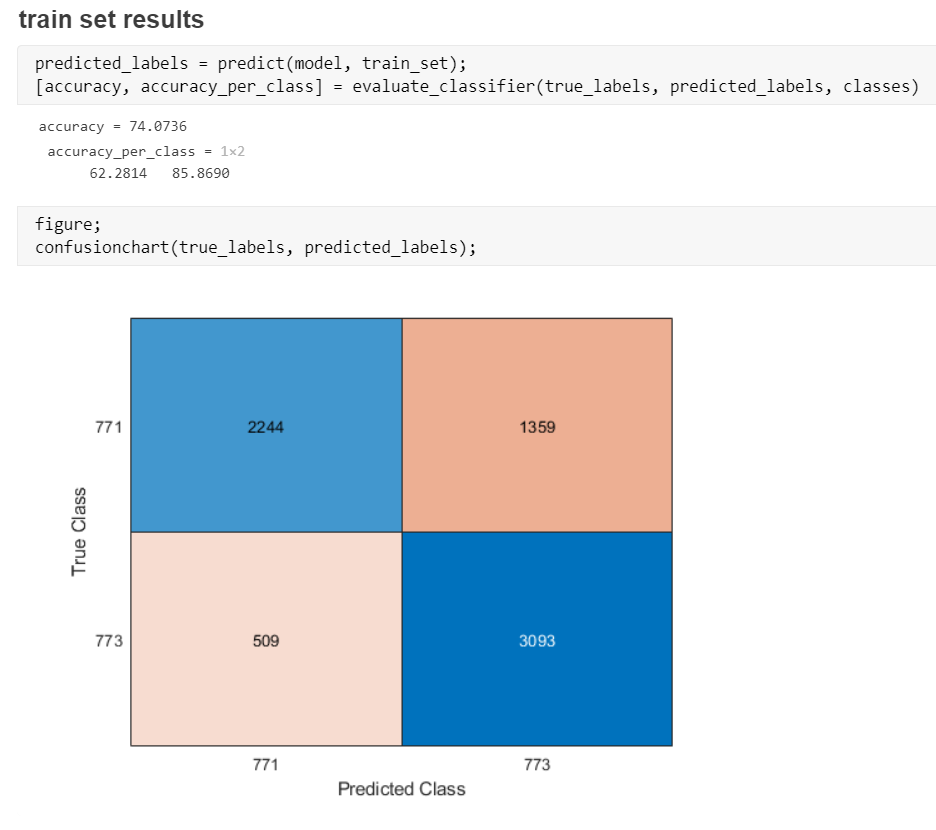
\includegraphics[width=0.7\linewidth]{img/code_train_set_results_ai6.PNG}
	\end{center}

	 \caption{Results of the trained classifier on training data (subject ai6)}
	 \label{fig:train_results_ai6}
\end{figure}


At the end of this step, for each subject we have a trained classifier, that takes in input the selected features from a window of the PSD, and returns in output the label of the MI task that it recognizes. \\
\item \textbf{Evidence accumulation tuning:} We also use offline data for tuning the parameters of the evidence accumulation frameworks that is used to obtain better classification at trial level. 
\end{itemize}

\noindent
{\Large\textbf{Online task:}}

\begin{itemize}
\item \textbf{Feature extraction:} Given the online data we extract from it the same features we found in the offline data for the subject (Figure \ref{fig:load_online_data_classifier_features_extraction}). 

\begin{figure}[h!]
	\begin{center}
		 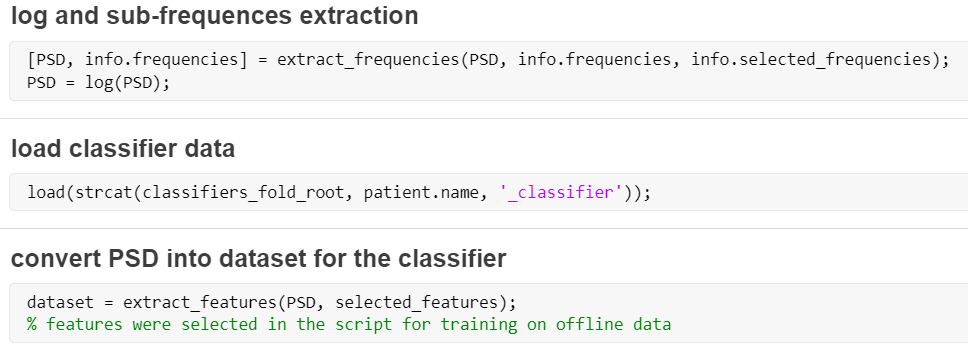
\includegraphics[width=0.7\linewidth]{img/code_load_online_and_features_extraction.PNG}
	\end{center}

	 \caption{Load of online data, trained classifier (for current subject), features  extraction}
	 \label{fig:load_online_data_classifier_features_extraction}
\end{figure}



\item \textbf{Classification test:} Once we have extracted the features, the classifier trained for the current patient is used to estimate the performed task, with a certain confidence value (Figure \ref{fig:test_results_ai6}). \\

\begin{figure}[h!]
	\begin{center}
		 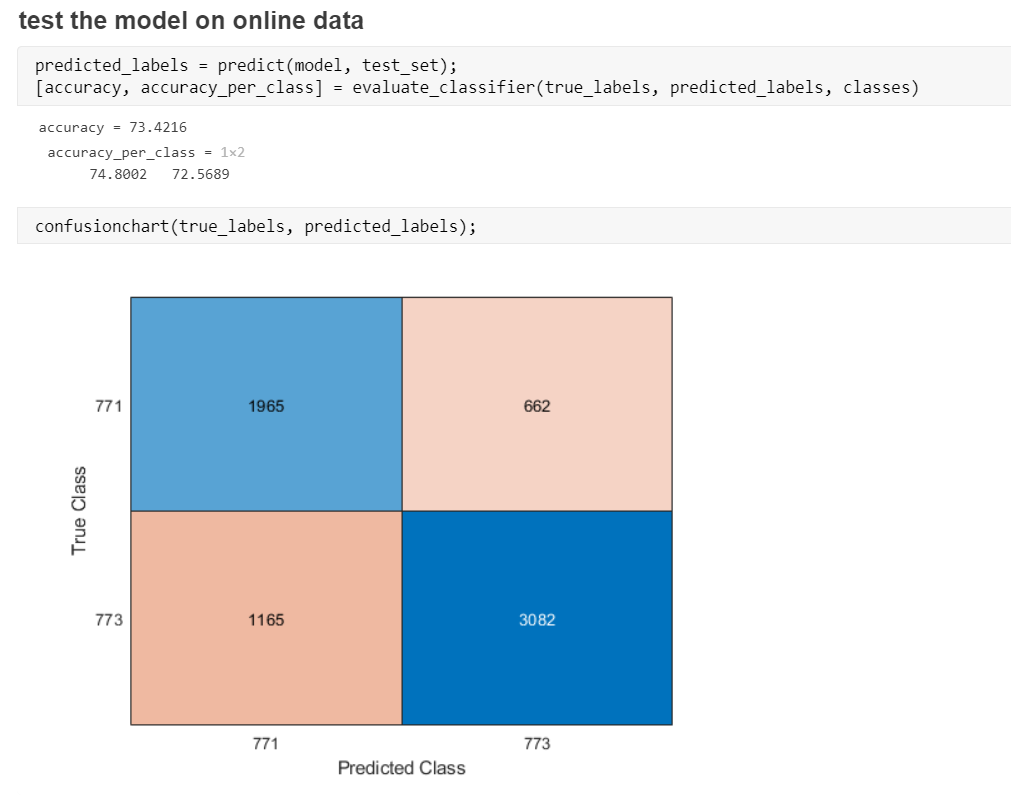
\includegraphics[width=0.7\linewidth]{img/code_test_set_results_ai6.PNG}
	\end{center}

	 \caption{Results of the trained classifier on test data (subject ai6)}
	 \label{fig:test_results_ai6}
\end{figure}

At last, we can evaluate the performance of the system with single-sample accuracy.
\item \textbf{Evidence accumulation test:} Then we use the evidence accumulation frameworks (with the parameters found in offline data for the subject) over the predictions of the classifier.\\
At the end we evaluate the performance on the continuos feedback period in order to obtain a trial level accuracy.
\end{itemize}